\section{Faltungen}

Seien $X,Y$ zwei reelle unabhängige Zufallsvariablen mit $X \sim \P_X$ und $Y \sim \P_Y$. Dann hat $(X,Y)$ die Verteilung $\P_X \otimes \P_Y$ auf $\R^2$. Anderseits ist auch $X+Y$ eine reelle Zufallsvariable, denn $X + Y = A(X,Y)$ für $\abb{A}{\R^2}{\R}$ mit $(x,y) \mapsto x+y$. $A$ ist stetig, also messbar. Die Verteilung von $X+Y$ ist dann $\brackets{\P_X \otimes \P_Y} \circ A^{-1}$.

\begin{definition}
	Seien $\P_1$ und $\P_2$ Wahrscheinlichkeitsmaße auf $(\Rn, \borel{\Rn})$. Das durch 
	\begin{equation*}
		\P_1 \ast \P_2 (F) \defeq \iint \one_F(x+y) \P_1(\mathrm{d}x) \P_2(\mathrm{d}y)
	\end{equation*}
	definierte Wahrscheinlichkeitsmaß $\P_1 \ast \P_2 = (\P_1 \otimes \P_2) \circ A^{-1}$ auf $(\Rn, \borel{\Rn})$ heißt \begriff{Faltung} von $\P_1$ und $\P_2$.
\end{definition}

\begin{satz} \label{3_25_satz}
	Seien $\abb{X,Y}{\Omega}{\Rn}$ unabhängige Zufallsvariablen mit Verteilungen $\P_X$ bzw. $\P_Y$. Dann ist 
	\begin{equation*}
		\P_{X+Y} = \P_X \ast \P_Y
	\end{equation*}
	die Verteilung von $X+Y$.
\end{satz}
\begin{proof}
	siehe Herleitung Faltung oben
\end{proof}

Faltungen von Wahrscheinlichkeitsmaßen mit Dichten besitzen wiederum eine Dichte.

\begin{proposition}
	Seien $\P_1$ und $\P_2$ Wahrscheinlichekeitsmaße auf $(\R, \borel{\R})$.
	\begin{enumerate}[leftmargin=*, nolistsep]
		\item \textbf{diskreter Fall:} Sind $\P_1$ und $\P_2$ de facto Wahrscheinlichkeitsmaße auf $(\Z, \pows{\Z})$ mit Zähldichten $\rho_1$ und $\rho_2$, dann ist $\P_1 \ast \P_2$ ein Wahrscheinlichkeitsmaß auf $(\Z, \pows{\Z})$ mit Zähldichte
		\begin{equation*}
			\rho_1 \ast \rho_2 (k) = \sum_{\ell \in \Z} \rho_1(\ell) \rho_2(k-\ell) \quad (k \in \Z)
		\end{equation*}
		\item \textbf{stetiger Fall:} Wenn $\P_1$ und $\P_2$ Dichtefunktionen $\rho_1$ und $\rho_2$ besitzen, dann besitzt $\P_1 \ast \P_2$ die Dichtefunktion
		\begin{equation*}
			\rho_1 \ast \rho_2 (x) \defeq \int_\R \rho_1(y) \rho_2(x-y) \dy \quad (x \in \R)
		\end{equation*}
	\end{enumerate}
\end{proposition}
\begin{proof}
	\begin{description}
		\item[Diskreter Fall:] Sei $k \in \Z$.
		\begin{equation*}
			(\P_1 \otimes \P_2) (A = k) = \sum_{\ell_1,\ell_2 \in \Z ; \ell_1 + \ell_2 = k} \rho(\ell_1)\rho(\ell_2) = \sum_{\ell,k \in \Z} \rho_1(\ell) \rho_2(k-\ell) = \rho_1 \ast \rho_2 (k)
		\end{equation*}
		\item[Stetiger Fall:] Sei $c \in \R$.
		\begin{equation*}
			\begin{aligned}
			\P_1 \ast \P_2 ((-\infty , c]) 
			&= (\P_1 \otimes \P_2)(A \le c) \\
			&= \int_\R \int_\R \one_{(\infty,c]}(x+y) \rho_1(x) \rho_2(y) \dx \dy \\
			\overset{y = z - x}&{=} \int_\R \int_\R \one_{(\infty,c]}(z) \rho_1(x) \rho_2(z-x) \dx \dz \\
			&= \int_{-\infty}^c \underbrace{\int_\R \rho_1(x) \rho_2(z-x) \dx}_{\rho_1 \ast \rho_2 (z)} \dz
			\end{aligned}
		\end{equation*}
	\end{description}
\end{proof}

\begin{beispiel}
	Seien $X \sim \Poisson(\lambda)$ und $Y \sim \Poisson(\mu)$ zwei unabhängige reelle Zufallsvariablen (mit Werten in $\N_0$). Dann ist $X+Y$ eine Zufallsvariable mit Werten in $\N_0$ und Zähldichte
	\begin{equation*}
		\begin{aligned}
		\P(X+Y = k) &= \sum_{\ell \in \Z} \P(X=\ell) * \P(Y=k - \ell) \\
		&= \sum_{\ell = 0}^k \frac{\lambda^\ell}{\ell !} e^{-\lambda} * \frac{\mu^{k-\ell}}{(k-\ell)!} e^{-\mu}
		= e^{-(\lambda+\mu)} \frac{1}{k!} \sum_{\ell = 0}^k \binom{k}{\ell} \lambda^\ell \mu^{k-\ell} \\
		&= e^{-(\lambda + \mu)} \frac{1}{k!} (\lambda + \mu)^k
		\end{aligned}
	\end{equation*}
	sodass $X+Y \sim \Poisson(\lambda + \mu)$, d.h. der Typ der Verteilung ist bei der Faltung erhalten geblieben. Das ist aber nicht immer der Fall.
\end{beispiel}

\begin{beispiel}
	Seien $X,Y \sim \Uni([0,1])$ zwei unabhängige Zufallsvariablen mit Dichten $\rho(x) = \one_{[0,1]}(x)$. Dann ist $X+Y$ eine Zufallsvariable mit Werten in $[0,2]$ und Dichte 
	\begin{equation*}
		\begin{aligned}
		\rho \ast \rho (x) 
		&= \int_{\R} \rho(y) \rho(y-x) \dy 
		= \int_{1 \land x} \one_{[0,1]}(y) \one_{[0,1]}(y-x) \dy 
		= \int_{1 \lor (x-1)} \dy \\
		&= \begin{cases}
			x & 0 \le x \le 1 \\
			2-x & 1 \le x \le 2 \\
			0 & \text{sonst}
		\end{cases}
		\end{aligned}
	\end{equation*}
	
	\begin{center}
		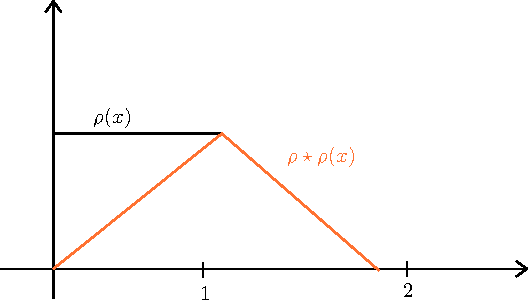
\includegraphics[width=.45\textwidth]{./stoch_abbildungen/faltung_dichte.pdf}
		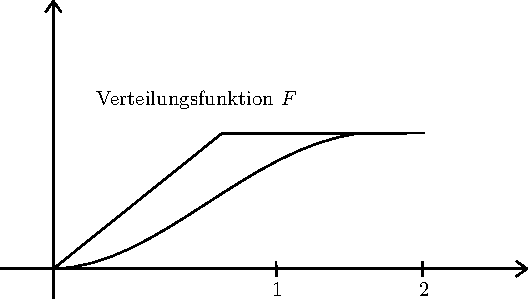
\includegraphics[width=.45\textwidth]{./stoch_abbildungen/faltung_verteilungsfunktion.pdf}
	\end{center}
	
\end{beispiel}